
\chapter{Introduction}

\label{chap:Introduction}


\section{The Oracle at Delphi}

On the eve of the second Persian invasion of Greece in the fifth century
BCE, the Oracle at Delphi prophesized the following to the people
of Sparta \citep{macauley}:

\begingroup     \fontsize{10pt}{12pt}\selectfont
\begin{quotation}
Hear your fate, O dwellers in Sparta of the wide spaces;

Either your glorious city must be sacked by the sons of Perses, 

Or, if it be not so, the whole land of Lacedaemon

Shall mourn the death of a king of the house of Heracles.
\end{quotation}
\endgroup

The Spartans, upon receiving this divination, ought to have understood
that their fortunes would likely deteriorate over the course of the
war, culminating in the loss of either their capital city or their
king (King Leonidas, a descendant of Heracles, and three hundred of
his men were driven to take a legendary last stand at Thermopylae
on the basis of this prophecy). It seems that the people of Sparta
learned something that day about the path of their fortunes over time,
not from the observations of data upon which much of modern statistical
inference is built, but rather from a fundamentally uncertain prognostication\textemdash what
we today might call a probabilistic forecast.

Modern probabilistic oracles, though perhaps less prescient than the
Oracle at Delphi, make forecasts in a great variety of domains. Moreover,
many of the variables over which these probabilistic forecasts are
generated can be modeled as stochastic processes. For example, the
distribution of expectations of professional forecasters for various
macroeconomic indicators over time are regularly reported by central
banks around the world. Meteorologists increasingly offer probabilistic
forecasts of everything from the path of cyclones to future humidity
and temperature levels, and market-determined distributions over the
prices of securities on future dates are implied by the prices of
options which expire on those dates (see \citet[Section II in][]{breeden-litzenberger-1978}).
If these forecasts reflect the truth, we can understand them as data
on the future distribution of a particular stochastic process, or
what we will refer to as distributional data. \figref{dist-data}
presents a intuitive visualization of a distributional datum, where
the value axis might represent any numeric value from the price of
a bond to a humidity reading. It ought to be kept in mind that the
depicted marginal distributions may be linked by some dependence structure
over time.

Some natural questions that can be asked of distributional data include:
\begin{aenumerate}
\item ``If we surveyed a group of economists for only their expectations
of one-year-forward inflation, what could we learn about their expectations
of six-months-forward inflation?'', or
\item ``Given the distribution of temperature in Boston a week from now,
what is the probability that the temperature in Boston tomorrow will
be higher than $15^{\circ}\mbox{C}$?'', or
\item ``How is the market pricing the distribution of a stock price between
dates on which the stock's associated options expire?''.
\end{aenumerate}
Though simple to pose, it is not clear what the mathematically rigorous
answers to general questions like these are.
\begin{figure}
\begin{centering}
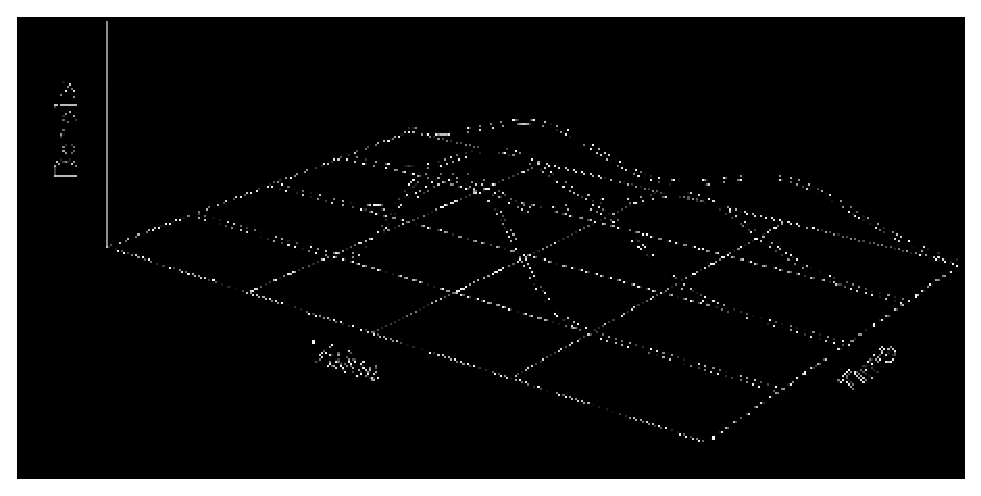
\includegraphics[width=0.5\columnwidth]{/Users/marshall/Documents/senior/thesis/figures/intuition_ed}
\par\end{centering}

\caption{\label{fig:dist-data}An intuitive depiction of a distributional datum.
This particular distributional datum is a four-dimensional joint distribution,
and the four marginal distributions of the data are shown at discrete
points in time.}
\end{figure}


This thesis rather focuses on answering two specific questions that
can be asked of a stochastic process when it is conditioned, in some
sense to be made precise in the next chapter, to follow a given distribution
at discrete future points in time. The first question is one of inference:
\begin{quote}
Can we, given distributional data and a parameterized stochastic process,
learn about the parameters governing the dynamics of the process? 
\end{quote}
The second is one of imputation:
\begin{quote}
Can we, given distributional data and a fully specified stochastic
process, impute the distribution of the process in between the times
at which it is conditioned?
\end{quote}
We will soon see that these questions of inference and imputation
are deeply related, and that the solution to either depends intimately
on the other. The answers to these specific questions allow us to
formulate a well-defined response to the broad questions about inflation,
weather, and stock prices posed above. These sorts of broad questions
abound; by extension, the potential applications of the methods proposed
here are both wide in scope and acute in importance. For instance,
one might imagine that knowing the market-implied distribution of
future stock prices could be immensely valuable. Moreover, references
to inference and imputation on distributional data in the context
of stochastic processes are sparse, if they appear at all, in the
literature. As such, this thesis represents the first investigation,
to the best of our knowledge, into inference on stochastic processes
when they are conditioned to follow a distribution at discrete future
points in time.


\section{Contributions and Related Work}

In the theoretical portion of this thesis, we propose a novel and
natural generalization of the theory of maximum likelihood estimation
over discretely observed data from continuous-time stochastic processes.
This theory begins with \citet{rao-1988} in general and \citet{yoshida-1992}
for the specific case of diffusion processes. In particular, we propose
that it is appropriate to use an estimator that minimizes Kullback-Liebler
(K-L) divergence for inference when given the distribution of a diffusion
process at discrete points in time. This is in contrast to the maximum
likelihood estimator, which is used for inference when given discrete
observations of such a process. We characterize this estimator as
a limiting case of the maximum likelihood estimator, and develop a
novel Monte Carlo expectation-maximization algorithm to conduct minimum
K-L divergence estimation, building on the work of \citet{beskos-2006}. 

However, this only partially answers the question of inference, since
the proposed procedure requires the ability to simulate a particular
generalized notion of a diffusion bridge. We therefore connect the
literature on the simulation of diffusion bridges (see \citet{bladt-sorensen-2014})
with the literature on generalized bridges (see \citet{baudoin-2002})
by proposing approximate and exact simulation strategies for a particular
class of generalized bridges. This answers in full the question of
inference. Simultaneously, we answer the question of imputation, having
gained the ability to draw sample paths of fully specified diffusion
processes whose endpoints are conditioned to follow a given distribution.

In the empirical portion of this thesis, we confirm the correctness
of the exact generalized bridge sampler. We further demonstrate that
the approximate sampler offers samples that are qualitatively similar
to those of the exact sampler at a fraction of the computation cost.
Then, we show empirically that the proposed simulation-based inference
technique on distributional data is unbiased for the K-L divergence
minimizing parameter. Moreover, we show that both the generalized
bridge samplers and the inference technique are robust to various
theoretical assumptions made in their derivations.

Finally, taking theory to practice, we use the proposed inference
scheme to estimate the parameters governing the evolution of inflation
expectations under diffusion models with and without analytically
tractable transition densities. We also propose an imputation scheme
for distributional data under a diffusion model specified only up
to its parameters. To conclude, we show that such a scheme, when applied
to probabilistic forecasts of inflation expectations, reduces the
out-of-sample K-L divergence of imputed distributions from true distributions
in a practically meaningful and statistically significant way relative
to linear interpolation.


\section{Outline}

The next chapter reviews the existing theory of stochastic bridges,
with emphasis on Markov bridges and the generalized bridges of \citet{baudoin-2002}.

With the mathematical underpinnings set, we present the theoretical
portion of this thesis in \chapref{EM} and \chapref{4}. \chapref{EM}
introduces and formalizes the problem of conducting inference on data
in the form of distributions. We propose an estimator for the parameters
governing a diffusion process when given distributional data and offer
interpretations of the resulting estimate in relation to the maximum
likelihood estimate; then, we develop a Monte Carlo expectation-maximization
algorithm which converges to the so-called minimum K-L divergence
estimate. We point out that a sampler for generalized diffusion bridges
is required to implement this algorithm, and in \chapref{4}, we present
approximate and exact versions of such a sampling scheme.

The theory developed in this thesis is applied in \chapref{5} and
\chapref{6}. We conduct a variety of simulations in \chapref{5}
to demonstrate both the correctness and robustness of the proposed
generalized bridge samplers and the Monte Carlo expectation-maximization
algorithm. In \chapref{6}, we synthesize and apply these methods
to model the inflation expectations of professional forecasters.

In \chapref{7}, we conclude and outline future directions for research.
